\documentclass{article}

\usepackage{ragged2e}
\usepackage{url}
\usepackage{bm}
\usepackage{graphicx}
\usepackage[ruled,linesnumbered]{algorithm2e}
%\usepackage{algpseudocode}
\usepackage{tabularx}
\usepackage{xcolor}
\usepackage{subcaption}
\usepackage{amsmath,amssymb,amsfonts}



\begin{document}

\begin{titlepage}
	\begin{center}
		{\Large\textbf{Technical Report}}\\ \large{\textbf{Upgradation from UGC-NET JRF to SRF}}
		\vspace{1cm}\\
            \textbf{RK Sanayaima Singh}\\
            \textbf{Reg. No. 21MCPC05}\\
		\vspace{1cm}
		\large Supervisors\\ 
		\large \textbf{Prof. Nagender Kumar Suryadevara}\\
		\vspace{1cm}
            \large DRC Members\\
            \large \textbf{Dr. Naveen Nekuri}\\
		\large \textbf{Dr. Odelu Vanga}\\
		\vspace{1cm}
        
\includegraphics[scale=1.5]{images/UoH.png} \\
        \vspace{0.5cm}
        \large School of Computer and Information Sciences \\
		\textbf{University of Hyderabad} \\
		Gachibowli, Hyderabad - 500 046 \\
		Telangana, India \\
		\vspace{0.5cm}
		\textbf{\today}
	\end{center}
\end{titlepage}



\large{\textbf{Status of the work from 19{th} October 2021 to date}}
\begin{enumerate}
    \item \normalsize{\textbf{Completed Course Work}}
    \begin{itemize}
        \item Research Methods in Computer Science - Core Course 
        \item Data Structures And Programming Lab - Core Course
        \item Algorithms - Core Course
        \item Research Publications and Ethics - Core Course
        \item Deep Learning - Elective Course
    \end{itemize}
%    \textcolor{red}{
%    \item \normalsize{\textbf{Survey of Visualization Recommendation and NLDR approaches}}
%    \begin{itemize}
%        \item Extensive survey on visualization recommendation and visualization selection approaches.
%        \item Extensive survey on NLDR approaches that visualizes the \sloppy{high-dimensional} data.
%    \end{itemize}
%}
    \item \normalsize{\textbf{Contributions}}

    \begin{itemize}
        \item \normalsize{\textbf{Contribution 1:}}\\
    \justifying{A 5G Edge-Deployed Digital Twin System for Automated Meibomian Gland Segmentation and Summarization}  paper drafted. %\textbf{Communicated to} IEEE Journal of Biomedical and Health Informatics

       \item \normalsize{\textbf{Contribution 2:}}\\
    Plan to propose an Agentic AI enabled automated segmentation and summarization of the meibomian glands.
    
    \end{itemize}

    \item \normalsize{\textbf{Conference Publications}}
    \begin{itemize}   
    \item 
    Singh, R.K.S., Suryadevara, N.K. (2023). \textbf{Causality Assessment for IIoT Sensing System and Digital Twin.} In: Suryadevara, N.K., George, B., Jayasundera, K.P., Mukhopadhyay, S.C. (eds) Sensing Technology. ICST 2022. Lecture Notes in Electrical Engineering, vol 1035. Springer, Cham. https://doi.org/10.1007/978-3-031-29871-4\_49

    \item M. Irfan, N. K. Suryadevara and R. S. Singh, \textbf{Comparative Analysis of Computer Vision and IMU Sensing Systems for Accurate Determination of Gait Parameters,} 2024 17th International Conference on Sensing Technology (ICST), Sydney, Australia, 2024, pp. 1-6, doi: 10.1109/ICST62759.2024.10992235.

    \item M. Kumari, R. S. Singh, N. K. Suryadevara and S. C. Mukhopadhyay, \textbf{A Learning Model for Hyderabad AQI based on Social Behaviour,} 2024 17th International Conference on Sensing Technology (ICST), Sydney, Australia, 2024, pp. 1-6, doi: 10.1109/ICST62759. 2024.10992226.
    
    \end{itemize}

    \item This report is organized as follows: Section 1 provides an introduction to meibomian gland and challenges. Section 2 presents the research objectives, concluding with a summary of the research work in Section 3 and future work in Section 4. 
    
\end{enumerate}
\newpage

\section{Introduction}

Meibomian Gland Dysfunction is a prevalent ocular surface disorder characterized by chronic abnormalities in the quantity or quality of meibum secretion, leading to evaporative dry eye ocular discomfort \cite{meiboworkshop}. Although very common, especially among ageing populations, accurate diagnosis and monitoring is challenging due to the variability in gland morphology and subjective nature of clinical assessment \cite{blackie2013symptoms}. Advancements in ocular imaging modalities such as high resolution infrared meibography makes automated and quantitative analysis of glandular structure possible \cite{arita2008meibography}. In parallel, semantic segmentation using deep learning has demonstrated remarkable performance in delineating fine-grained anatomical features in biomedical images \cite{ronneberger2015unet}. However, the translation of these techniques into clinically usable systems remains limited due to the lack of personalization, system-level feedback, and real-time adaptability.


%\begin{table*}[htpb]
%    \centering
%    \begin{tabularx}{\linewidth}{l|X|X}
%        \hline
%        Physical Entity & Mechanism & Endpoint \\
%        \hline
%        Lung \cite{lexma} & Blood and oxygen flow simulation & Predict ventilation requirements \\    
%        Heart \cite{BAILLARGEON201438} & Simulate the structure and physiologic function of the heart & Customization and optimization of cardiac devices \\
%        Heart \cite{seimens} & Simulates the structure and physiologic function of the heart & Cardiac resynchronization \\
%        Heart \cite{Obaid2019} & Simulated TAVR implantations with different aortic prosthesis & Surgical planning \\
%        Spine \cite{Ahmadian2022} & Predict Vertebral Fracture after Stereotactic Body Radiotherapy & Optimal radiation plan to minimize treatment side effects \\
%        Alzheimer’s disease \cite{Fisher2019}& Predicting the individual outcome in neurological diseases & DT of controls of clinical trial and ultimately clinical interventions \\
%        Breast lesions \cite{Badano2018}  & mage based virtual patients comparing digital mammography to tomosynthesis & Determine which imaging tool is better at detecting breast lesions \\
%        Type 2 Diabetes \cite{cleaveland} & Disease reversal in type 2 diabetes  & Randomized control trial examining twin precision treatment vs. standard of care \\
        
%        Meibomian Gland & Semantic segmentation and LLM based analysis and reporting & Gland degradation grading, workflow (this work) \\
%        \hline
%    \end{tabularx}
%    \caption{Comparision of various DT for healthcare \cite{Katsoulakis2024}}
%    \label{tab:dt_comparision_table}
%\end{table*}


Eye-related diseases encompass a wide range of conditions affecting ocular health, with Meibomian gland dysfunction (MGD) being one of the most prevalent. MGD is characterized by abnormalities in the meibomian glands, leading to terminal duct obstruction and alterations in meibomian gland secretions. This dysfunction is a significant contributor to dry eye symptoms and is implicated in various ocular surface diseases worldwide, affecting millions of individuals and impacting their quality of life \cite{meiboworkshop}. MGD is multifactorial, its severity influenced by environmental conditions such as air pollution and humidity, as well as intrinsic factors like hormonal fluctuations and systemic diseases. The pathophysiology of MGD involves glandular obstruction and potential atrophy, often exacerbated by incomplete blinking and muscle dysfunction surrounding the meibomian glands. The glandular obstruction results in a compromised tear film and tear evaporates at a much faster rate. Rapid tear evaporation leads to symptomatic dry eye disease.

In the early stages of MGD, the symptoms may be minimal. However, physical signs such as meibomian gland dropout and abnormalities in lid margin can be observed. Such abnormalities can be evaluated through imaging techninques such as infrared meibography. MGD coexists with various ocular and systemic diseases which makes the diagnosis and management complicated. Clinical diagnosis of MGD typically is a combination of patient-reported symptoms with objective assessment and classifying into several stages of severity. The ocular surface health is examined through various methods such as Ocular Surface Disease Index (OSDI), tear meniscus height (TMH), and tear break-up time (TBUT). Treatment of MGD is generally additive and depends on the severity of it. A patient diagnosed with Stage 3 MGD may receive interventions indicated for Stages 1 and 2 as well. Therapeutic treatment aims at alleviating symptoms and restoring normal gland function which ranges from artificial tear and anti-inflammatory medications to thermal pulsation treatment and meibomian gland expression \cite{geerling2011management}.

While AI-driven tools like semantic segmentation and large language models (LLMs) automate and standardize diagnostics, existing solutions in ophthalmology are isolated  with segmentation models operating independently of clinical workflows and LLMs are underutilized for diagnostic summarization. %Digital twin technology addresses these limitations by enabling continuous interaction between physical data, computational models, and decision-support layers. Digital twin technology—a dynamic, virtual representation of physical entities—has emerged as a promising paradigm in healthcare to address these gaps by enabling real-time simulation, monitoring, and predictive diagnostics \cite{fuller2020digital}. While digital twins have seen successful applications in cardiology \cite{corral2020digital}, oncology \cite{bruynseels2018ethics}, and orthopedic modeling \cite{viceconti2018digital}, their potential in ophthalmology, particularly for glandular dysfunctions, remains largely unexplored. A brief comparison of such systems is shown in table \ref{tab:dt_comparision_table}. Several works in the AI-enabled digital twins are working toward applying diverse methods such as neuro-symbolic AI, Quantum Federated Learning, etc. in the clinical decision making \cite{neurosymbolicdt} \cite{digitaltwin5g} \cite{decidetwin}.



\subsection{Challenges}

\begin{itemize}
    \item The complexity in meibomian gland morphology exhibit irregular shape, length and different degree of visibility. Accurate semantic segmentation is required to view the glandular structures.
    \item Manual analysis of infrared meibography may be subject to inter-observer variability due to differences in clinical expertise and individual interpretation. An automated baseline analysis is required to support the assessment of meibography images.
    
    %\item Develop an LLM-enabled Digital Twin for the meibomian gland analysis and summarization.
    %\item Deploying the 
\end{itemize}

\section{Research Objectives}
\begin{itemize}
    \item To develop U-Net-based semantic segmentation modules for the automated segmentation of meibomian gland and eyelid regions using the MGD1k dataset.
    \item To integrate the MedGemma large language model (LLM) for analyzing segmentation-derived information and generating structured, interpretable reports.
    \item To deploy the developed segmentation and LLM-based reporting modules on a 5G MEC testbed and evaluate their functionality within the target application environment.
\end{itemize}


%\subsection{Incremental Visualization Recommendation based on Intent}
 \section{Methods}
The methodology consists of four major components: (i) data used for training and testing, (ii) model selection for gland and eyelid segmentation, (iii) application pipeline, (iv) fine-tuning an LLM. We have developed an attention U-Net based segmentation model and fine tuned a vision-language  LLM\cite{vaswani2017attention} to be integrated into the system.


\subsection{Dataset}

The study utilized a dataset of infrared meibography images named 'MGD-1K'\cite{saha2022automated}. The dataset was collected at Yeouido St. Mary's Hospital over a one-year period. The dataset id openly accessible at \url{https://mgd1k.github.io/}

MGD-1k consists of 1000 infrared meibography images acquired from 320 patients using the non-contact infrared imaging function of the LipiView II Ocular Surface Interferometer (Johnson \& Johnson Inc., Jacksonvile, FL). The patient cohort has a mean age of 54.6 $\pm$ 20.2 years and includes 107 men (33.4\%) and 213 women (66.6\%) gland (MG) images. This provides diverse sample for evaluation.

The dataset contains images from both eyelids. A total of 467 upper-eyelid images and 533 lower-eyelid images are available. Each image is accompanied by corresponding eyelid and meibomian gland segmentation masks. These masks serve as the ground truth for model training and evaluation. An example of the infrared meibography image with its corresponding eyelid and gland masks is presented in Figure \ref{fig:meibography_example}.

\begin{figure}[h]
    \centering
    \begin{subfigure}{0.32\columnwidth}
        \centering
        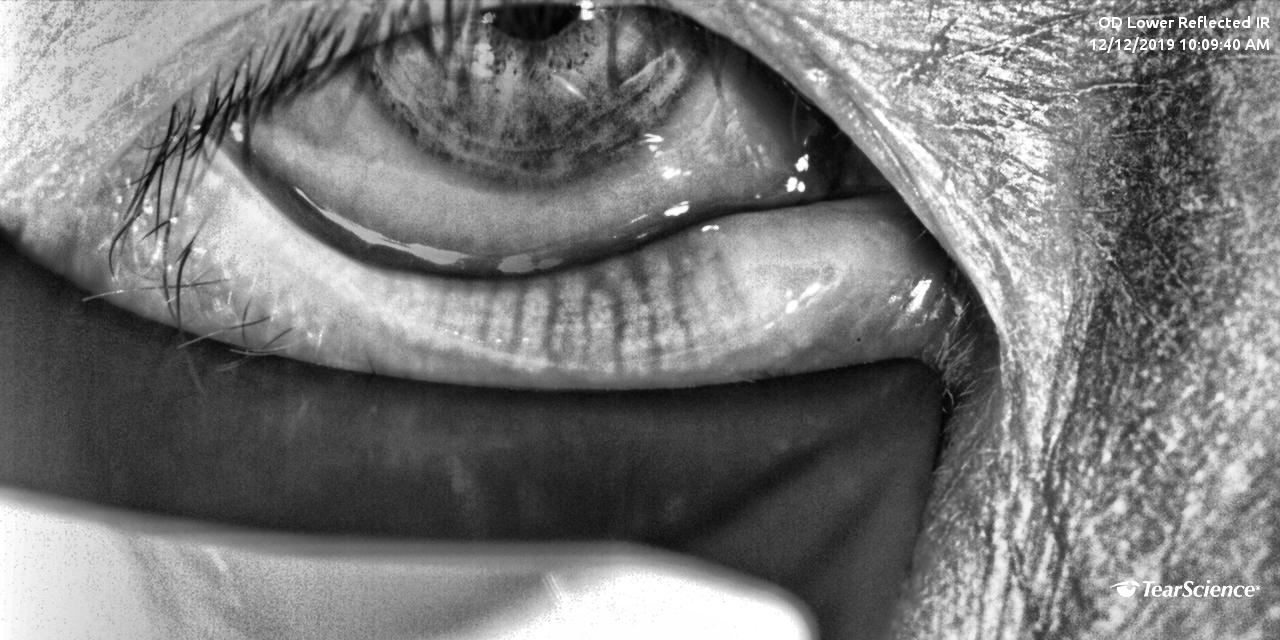
\includegraphics[width=\linewidth]{singh1.jpg}
        \caption{IR image}
        \label{fig:meibography_image}
    \end{subfigure}
    \begin{subfigure}{0.32\linewidth}
        \centering
        
\includegraphics[width=\linewidth]{singh2.png}
        \caption{Eyelid mask}
        \label{fig:eyelid_mask}
    \end{subfigure}
    \begin{subfigure}{0.32\linewidth}
        \centering
        
\includegraphics[width=\linewidth]{singh3.png}
        \caption{Gland mask}
        \label{fig:gland_mask}
    \end{subfigure}

    \caption{Example images from the MGD1k dataset. (a) Meibography image showing the meibomian glands in the eyelid. (b) Eyelid mask highlighting the region of interest. (c) Gland mask indicating the segmented meibomian glands.}
    \label{fig:meibography_example}
\end{figure}

\subsection{Model selection}

Accurate image segmentation is a crucial task in medical image analysis to enable quantitative and computer-aided analysis. Traditional manual diagnosis which relies heavily on expert knowledge can not scale with the challenges of increasing volume of medical image data. This necessity calls for automated methods to improve efficiency and reduce workload. Medical images such as computed tomography (CT), magnetic resonance imaging (MRI), ultrasound and X-Rays have unique difficulties in automated segmentation  due to blurred boundaries, low-contrast tissue environments and noise like speckle in ultrasound. The U-Net architecture, introduced by Ronneberger \textit{et al.} in 2015 have emerged as a very successful model for biomedical image segmentation \cite{ronneberger2015unet}. The encoder-decoder design and skip connections of U-Net effectively preserve spatial information while capturing precise localization of anatomical structures. Conventional skip connections transmit all encoded features to the decoder, including redundant or irrelevant responses which may adversely affect segmentation performance.

Recent advances in attention mechanisms have shown the effectiveness of selectively emphasizing informative features while suppressing the less relevant ones. This improves the modelling of contextual information \cite{vaswani2017attention}. Oktay \textit{et al.} incorporated Attention Gates (AGs) into the U-Net architecture to selectively filter encoder features before they are fused with the decoder \cite{oktay2018attention}. This adaptive feature selection enables the network to focus on anatomically relevant regions without introducing significant computational overhead.


Attention U-Net is particularly well suited to infrared meibography, where gland structures are often difficult to distinguish because of uneven illumination, low tissue contrast, imaging artifacts, and substantial morphological variation. By enhancing discriminative gland features while suppressing background responses, the attention gates improve the delineation of both the eyelid boundary and individual meibomian glands. Based on these considerations, Attention U-Net was selected as the segmentation model for this study.

\subsection{Training}

A subset of the MGD-1k dataset \cite{saha2022automated} was used to train both the segmentation models. The subset contains 941 annotated meibography images. The dataset was split into 80:20 training-validation ratio which makes 752 training images and 189 validation images. The images were resized to $512 \times 512$ pixels and normalized. The segmentation models were trained using the corresponding ground truth masks for eyelid and the gland for 20 epochs each.

The U-Net model is trained on the dataset using several loss functions. For empirical evaluation, we have used region-based metrics like the Dice Similarity Coefficient Loss \cite{milletari2016vnet} and Tversky Loss \cite{salehi2017tversky}, standard classification metrics such as Binary Cross-Entropy (BCE) and Focal Loss \cite{lin2017focal}, boundary-focused Contour Loss \cite{clason2013convex}, and hybrid approaches including Combo Loss (Dice + BCE) \cite{taghanaki2019combo} and IoU + BCE Loss \cite{rahman2016optimizing}. Both the eyelid and gland segmentation models are trained independently on the dataset using each of the loss functions.
%Table \ref{t} 

Performance was evaluated using the Dice Similarity Coefficient (DSC), Intersection over Union (IoU), and pixel-wise accuracy on the validation set. To monitor training dynamics, loss curves for eyelid and gland segmentation were recorded and are presented in Figure \ref{fig:training_loss}.

\begin{figure}
    \centering
    
    \begin{subfigure}{\columnwidth}
        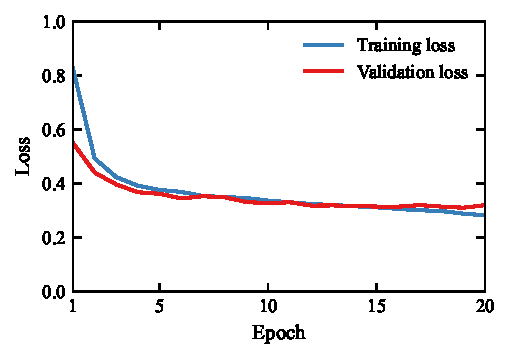
\includegraphics[width=\linewidth]{singh4.pdf}
        \caption{Gland Segmentation Loss}
        \label{fig:gland_loss}
    \end{subfigure}
    \begin{subfigure}{\columnwidth}
        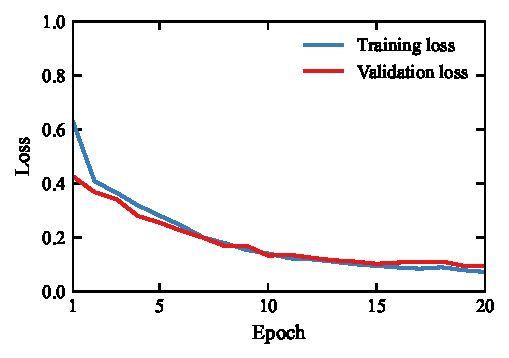
\includegraphics[width=\linewidth]{singh5.pdf}
        \caption{Eyelid-region Segmentation Loss}
        \label{fig:eyelid_region_loss}
    \end{subfigure}
    \caption{Training loss curves for the gland and eyelid region segmentation tasks. The plots show the loss values over the training epochs, indicating the convergence of the model during training.}
    \label{fig:training_loss}
\end{figure}


\subsection{Fine tuning a large language model}
A large language model (LLM) is fine-tuned to generate summarization reports based on the input meibography images. The LLM is trained on the MGD1k dataset. During the training process, the 1,000 meibography images are paired with their corresponding meiboscore grading. The grading is converted to a text format that describes the meiboscore in a structured manner. The choice of words is taken to reduce the token similarity of the descriptions. This text format is used as the target output for the LLM during training.

The LLM taken is the MedGemma \cite{sellergren2025medgemma} model, which is a large language model specifically designed for medical applications. It is based on Google Gemma architecture and has been fine-tuned on a diverse range of medical images including x-ray, radiology, and ophthalmological images. The model is capable of understanding complex medical terminology and generating coherent and contextually relevant text. The MedGemma vision-language model is fine-tuned to classify and summarize the meibomian gland dropout in infrared meibography images.

%The dataset preparation for fine-tuning, prompt formulation, the parameter0efficient fine-tuning (PEFT) strategy are as follows.

\subsubsection{Dataset and Preprocessing}
The MGD1K \cite{saha2022automated} dataset used to train the segmentation models is further used to fine tune the LLM. The primary task is to classify the severity of gland dropout into one of four categories. The dataset was partitioned into training and validation set with as fixed seed to ensure reproducibility. The split consisted of 759 samples for training and 189 samples for validation. Each data point is formatted as an image (as a PIL object) and its corresponding integer label from 0 to 3 

%(\textit{seed=42})%
\subsubsection{Model Architecture and Prompt Formulation}
The foundation model for the experiment is the \textbf{MedGemma} (\texttt{google /medgemma-4b-it}) model. We have taken the 4-billion parameter, instruction-tuned version. MedGemma is provided as a pre-trained Vision Language Model by Google for biomedical applications. To adapt this model to our specific classification task, we formulated the problem as a multiple-choice question answering task \cite{sellergren2025medgemma}.

A standardized textual prompt was designed to help classify the image into labels. The prompt instructs the model to select the most fitting description of the gland dropout out of the four options provided, each corresponding to an integer class label. The four integer class labels of classification categories were also described with text to provide clear, qualitative anchor for the model:

\begin{enumerate}
    \item[\textbf{A.}] Intact, Pristine, Barely affected (Label 0)
    \item[\textbf{B.}] Mildly compromised, Early signs of damage, Partial impairment (Label 1)
    \item[\textbf{C.}] Marked deterioration, Substantial decline, Advanced impairment (Label 2)
    \item[\textbf{D.}] Severe degradation, Profound damage, Near-total loss (Label 3)
\end{enumerate}

The final prompt ($P$) presented to the model was structured as follows: $P = $ "\texttt{What is the most likely gland dropout rate shown in the infrared meibomian gland image?\textbackslash n A. ...\textbackslash n B. ...\textbackslash n C. ... \textbackslash n D. ...}. Each data sample was formatted into a conversational structure with a \texttt{user} role (containing the image and the prompt $P$) and an \texttt{assistant} role (containing the ground-truth text answer corresponding to the image's label). This formatting was done to align with the instruction-tuning paradigm of the base MedGemma model.

\subsubsection{Parameter-Efficient Fine-Tuning (PEFT) with QLoRA}
To efficiently fine-tune the 4-billion parameter model on commodity hardware, we employed the \textbf{Quantized Low-Rank Adaptation (QLoRA)} technique \cite{hu2021loralowrankadaptationlarge} \cite{dettmers2023qlora}. QLoRA enables significant memory savings by quantizing the pre-trained model to 4-bits and then training a small number of adaptable parameters.

\textbf{Low-Rank Adaptation (LoRA)} module is integrated to freeze the original pre-trained model weights ($W_0 \in \mathbb{R}^{d \times k}$) and injects a pair of trainable, low-rank matrices ($A \in \mathbb{R}^{r \times k}$ and $B \in \mathbb{R}^{d \times r}$), where the rank $r \ll \min(d, k)$. The forward pass is modified as shown in Equation \ref{eq:lora}, where the output of the LoRA adapter, scaled by a factor $\alpha$, is added to the output of the frozen pre-trained layer.

\begin{equation}
\label{eq:lora}
h = W_0x + \Delta Wx = W_0x + \frac{\alpha}{r}BAx
\end{equation}

The specific LoRA configuration for our experiment was as follows:
Rank ($r$): 16, Alpha ($\alpha$): 16, Dropout: 0.05, Target Modules: All linear layers within the model architecture (\texttt{all-linear}). 

\subsubsection{Training and Optimization}
The fine-tuning process was managed using the \texttt{SFTTrainer} from the Hugging Face TRL library \cite{trl}. The training was configured with the following hyperparameters: Epochs: 5, Learning Rate: $2 \times 10^{-4}$, Optimizer: Fused AdamW (\texttt{adamw\_torch\_fused}). Gradient checkpointing was enabled to reduce VRAM consumption.


A custom data collator function was implemented to process batches. This function tokenizes the text prompts and prepares the images for the model. Crucially, for loss computation, the labels are derived from the input token IDs. The loss mask was designed to ignore padding tokens, the special image token (\texttt{<image>}), and other non-textual tokens, ensuring that the backpropagation signal was computed solely based on the model's ability to predict the correct textual answer (e.g., "B. Mildly compromised..."). Evaluation was performed every 50 steps on a shuffled subset of 200 samples from the validation set.

\subsection{Digital Twin System workflow}
The system pipeline is designed to simulate the clinical diagnosis of meibography image. The system allows users to upload meibography images, which are then processed by the segmentation modules to generate gland and eyelid masks. The large language model (LLM) is used to create a summary of the images. The workflow is illustrated in Figure \ref{fig:dt_sequence_diagram}.
\begin{figure}[ht]
    \centering
    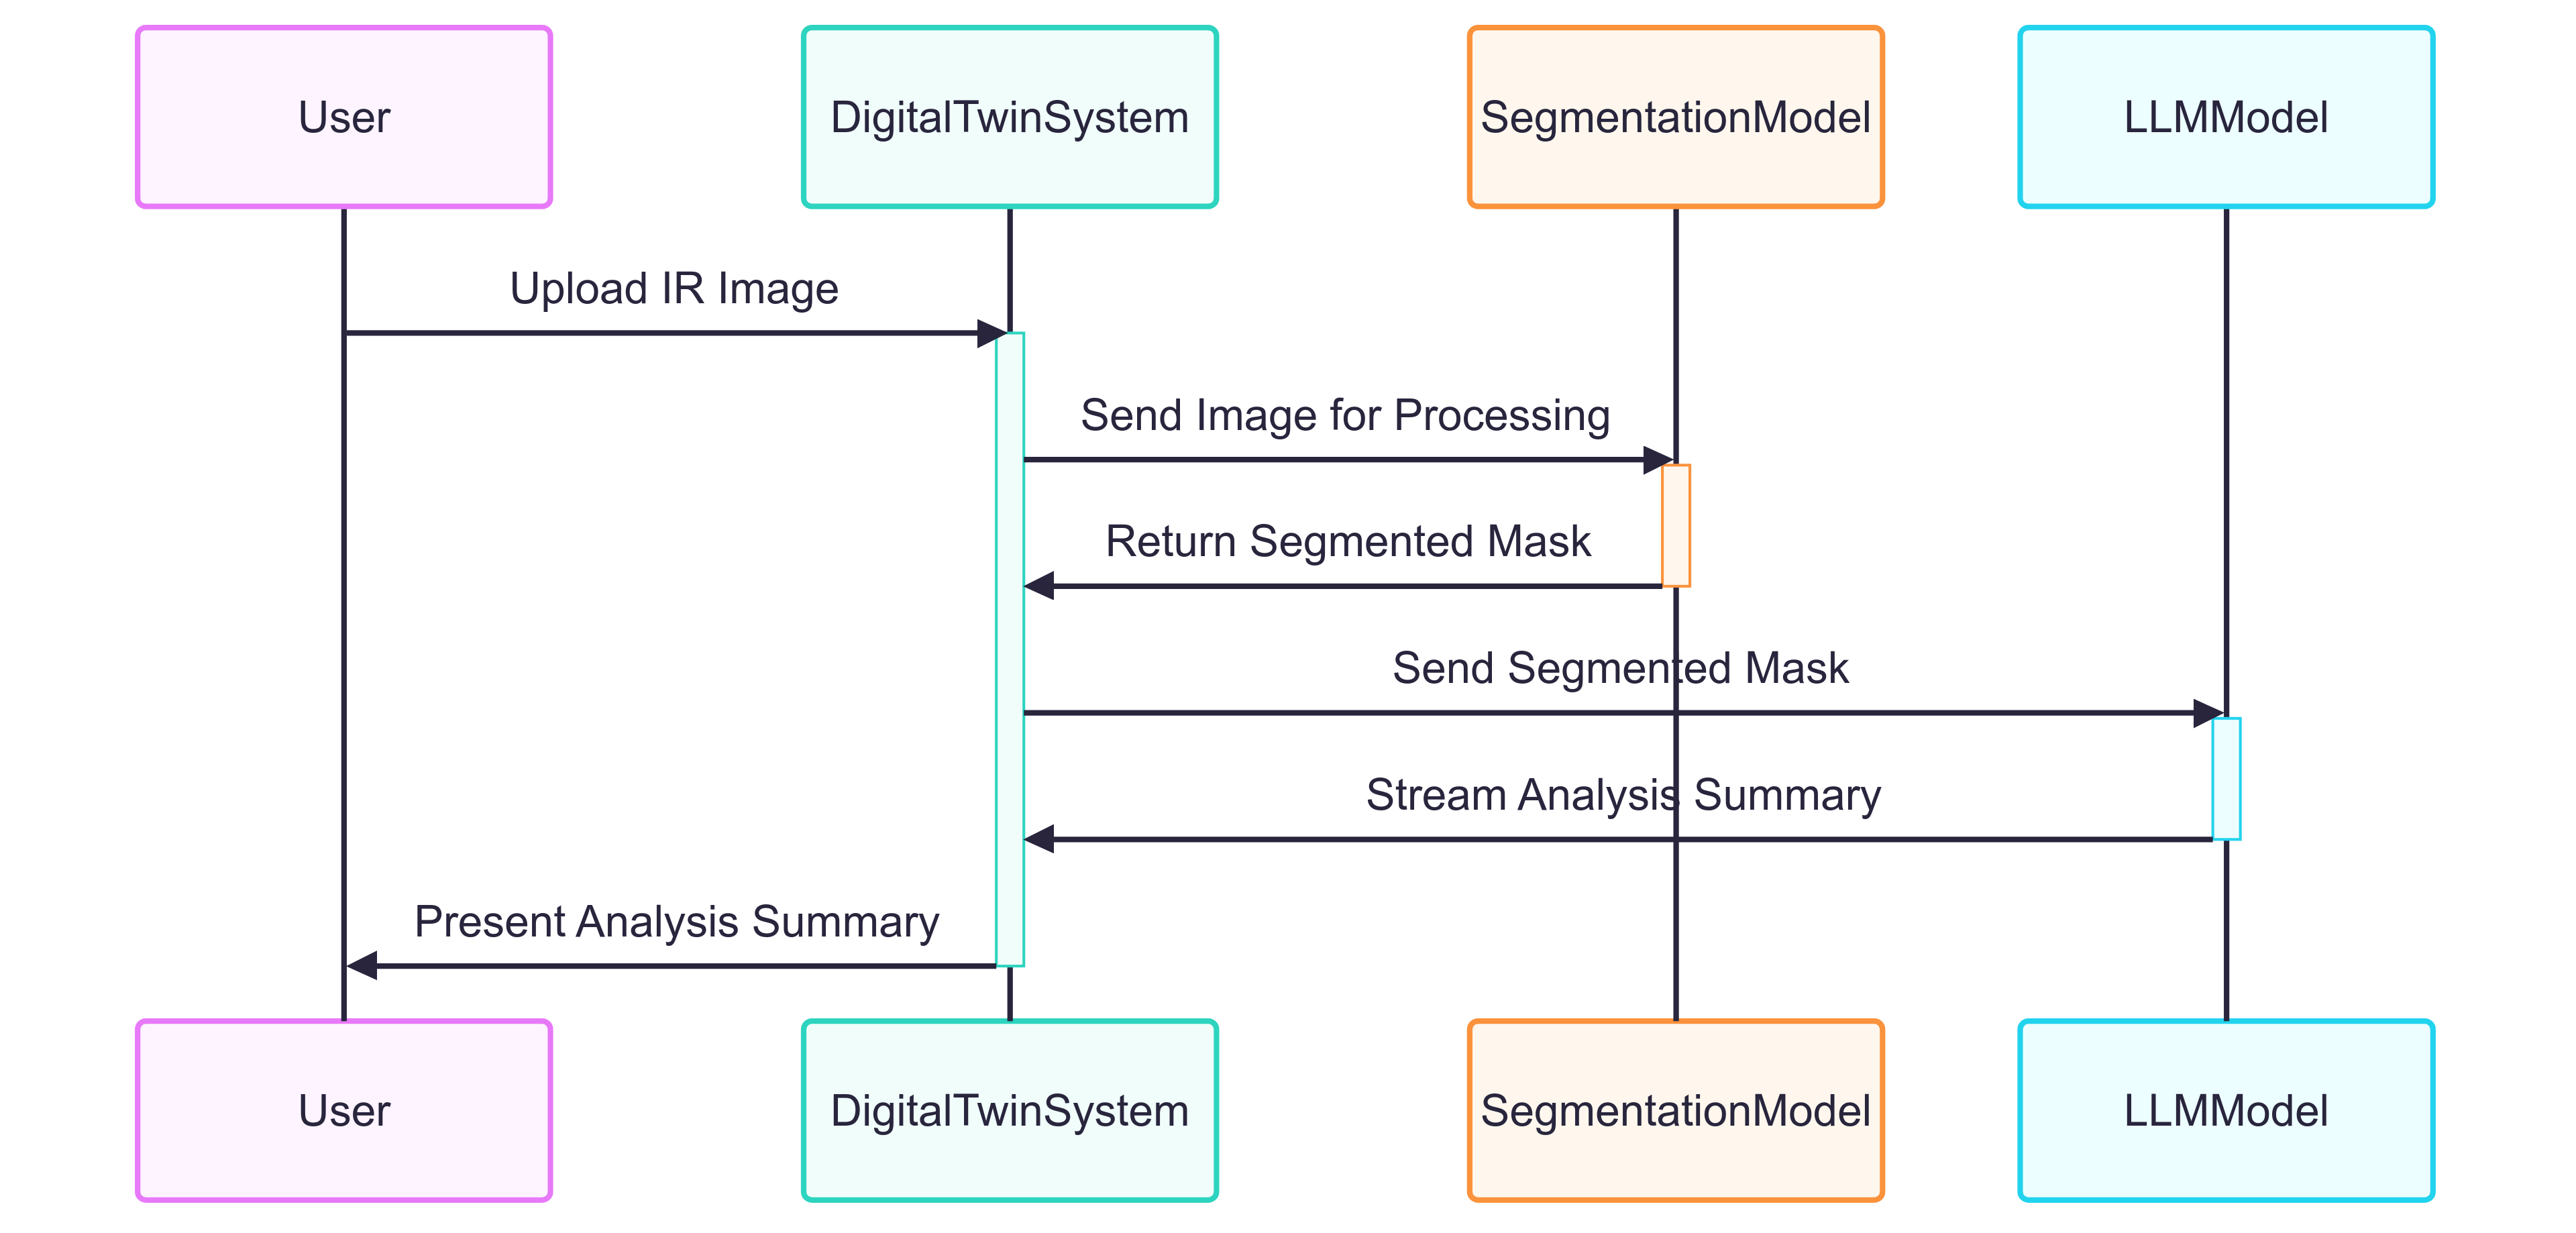
\includegraphics[width=\linewidth]{singh6.png}
    \caption{Sequence diagram of the Digital Twin. The diagram illustrates the interactions between the user, the segmentation module, and the large language model (LLM) for generating diagnostic reports.}
    \label{fig:dt_sequence_diagram}
\end{figure}

The Digital Twin workflow incorporates an interactive user interface engineered to emulate and analyze diagnostic workflows in meibomian imaging. The analytical pipeline starts by loading an infrared meibography image. The image may undergo an optional preprocessing stage to enhance feature visibility. This preprocessing stage utilized the Contrast-Limited Adaptive Histogram Equalization (CLAHE) algorithm \cite{pizer1987adaptiveclahe}. The user is allowed to set the CLAHE parameters i.e. the clip limit, which modulates the degree of local enhancements and the grid size, which is the dimension of the regional tiles for equalization. These parameters help in preprocessing for better glandular structure delineation and mitigate the amplification of stochastic noise.

Following the optional preprocessing step, the pipeline passes the image to two separate pre-trained segmentation models. One module isolates the region of interest by creating a binary mask of the eyelid which delineates the anatomical boundary. The other performs the meibomian gland segmentation by specifically targeting the glandular structure within the tarsal plane and creating a precise binary mark of the gland structure. The physical object i.e. the meibomian gland is brought to the virtual environment as infrared meibography imagery. To close the physical-to-virtual feedback loop, the system displays the resulting binary masks, both the eyelid and the gland masks, concurrently. An optional overlay visualization is provided to manually check the segmentation accuracy. This overlay function renders a composite image by superimposing the masks onto their original source image with an alpha transparency of 0.5. The display of this overlay alongside the masks provides a visual feedback mechanism which allows for direct validation of the segmentation results against the underlying anatomical context. The working of the Digital Twin is formalized in algorithms \ref{alg:meibomian_gland_segmentation_and_summarization}, \ref{alg:meibomian_gland_segmentation}  and \ref{alg:llm_invocation}. This Digital Twin workflow serves as a simulation of real-time diagnostic support in an ophthalmic setting.


%\begin{algorithm}
%    \caption{Algorithm for Meibomian Gland Segmentation and Report Generation}
%    \label{alg:meibomian_gland_segmentation_and_summarization}
%    \begin{algorithmic}[1]
%        \State \textbf{Input:} Meibography image $I$
%        \State \textbf{Output:} Segmented gland mask $M_g$, Eyelid mask $M_e$, Diagnostic report $R$

%        \State $M_g, M_e \gets \text{Attention U-Net}(I)$
%        \State $R \gets \text{LLM}(M_g, M_e)$

%        \Return $M_g, M_e, R$
%    \end{algorithmic}
%\end{algorithm}

%

\begin{algorithm}[H]
    \caption{Algorithm for Meibomian Gland Segmentation and Report Generation}
    \label{alg:meibomian_gland_segmentation_and_summarization}

    \KwIn{Meibography image $I$}
    \KwOut{Segmented gland mask $M_g$, eyelid mask $M_e$, diagnostic report $R$}

    $M_g, M_e \gets \operatorname{AttentionUNet}(I)$\;

    $R \gets \operatorname{LLM}(M_g, M_e)$\;

    \Return{$M_g, M_e, R$}

\end{algorithm}

%=============

\begin{algorithm}[H]
\caption{Workflow for IR Meibography Segmentation}
\label{alg:meibomian_gland_segmentation}

\KwIn{Grayscale IR meibography image $I$}
\KwOut{Eyelid mask $M_{\mathrm{eyelid}}$, gland mask $M_{\mathrm{gland}}$, and optional overlay $O$}

Upload grayscale IR meibography image $I$\;

Display option: \textbf{Apply Preprocessing? (Yes/No)}\;

\eIf{User selects Yes}{
    Request user input: CLAHE clip limit $c$ and grid size $g$\;
    
    $I_{\mathrm{pre}} \gets \operatorname{CLAHE}(I,c,g)$\;
}{
    $I_{\mathrm{pre}} \gets I$\;
}

$M_{\mathrm{eyelid}} \gets
\operatorname{EyelidSegmentation}(I_{\mathrm{pre}})$\;

$M_{\mathrm{gland}} \gets
\operatorname{GlandSegmentation}(I_{\mathrm{pre}})$\;

Display $M_{\mathrm{eyelid}}$ and $M_{\mathrm{gland}}$ as binary images\;

Display option: \textbf{Show Overlay? (Yes/No)}\;

\If{User selects Yes}{
    $O \gets \operatorname{Overlay}
    (I,M_{\mathrm{eyelid}},M_{\mathrm{gland}},\alpha=0.5)$\;
    
    Display $O$ beneath $M_{\mathrm{eyelid}}$ and $M_{\mathrm{gland}}$\;
}

\end{algorithm}
%=============


\begin{algorithm}[H]
    \caption{Inference Pipeline using Fine-Tuned \texttt{medgemma-mgd1k} Model}
    \label{alg:llm_invocation}

    \KwIn{IR meibography image $I$, fine-tuned model $\mathcal{M}$, processor $\mathcal{P}$, prompt $\mathcal{Q}$}
    \KwOut{Generated classification output $Y$}

$I_{rgb} \gets \text{ConvertToRGB}(I)$\;

$M \gets \texttt{[User, System]}$ chat message template with $I_{rgb}$ and prompt $\mathcal{Q}$\;

$X \gets \mathcal{P}.\text{apply\_chat\_template}(M,$
\texttt{add\_generation\_prompt=True})$\;

$T \gets \mathcal{P}.\text{tokenize}(X,\texttt{return\_tensors="pt"})$\;

$T \gets T.\text{to}(\texttt{device},\texttt{dtype=torch.float16})$\;

$n \gets \text{Length}(T[\texttt{"input\_ids"}])$\;

$\hat{Y} \gets \mathcal{M}.\text{generate}(T,\texttt{max\_new\_tokens}=200)$\;

$Y \gets \mathcal{P}.\text{decode}(\hat{Y}[0][n:],\texttt{skip\_special\_tokens=True})$\;

\Return{Y}\;

\end{algorithm}

\subsection{Deployment and Interface Integration in 5G MEC Server}

The Digital Twin system is designed and deployed in a 5G test bed. The modules of the Digital Twin are deployed on the edge i.e. the 5G Multi-Access Edge Computing Server. Several studies 
have shown the advances of 5G in healthcare \cite{5gdiabetes} \cite{5gafrica} \cite{5gprakash}. The proposed architecture functions as a localized Digital Twin system, mapping the physical diagnostic workflow—capturing infrared meibography—into a synchronized virtual environment. When multiple User Equipments (UEs) concurrently transmit high-resolution meibography images, traditional cloud-based architectures suffer from severe uplink saturation and queuing delays. Our approach circumvents this by localizing the computational workload at the network edge. The physical-to-virtual loop is facilitated by a local 5G network terminating at an on-premise MEC server providing an Ubuntu virtual machine. The 5G network ensures that large infrared image payloads from UEs are transmitted to the server with sub-millisecond network latency. Keeping the diagnostic data loop entirely on-premise ensures compliance with medical data regulations while preventing external internet bandwidth fluctuations from impacting the user experience.

\begin{figure}[h]
    \centering
    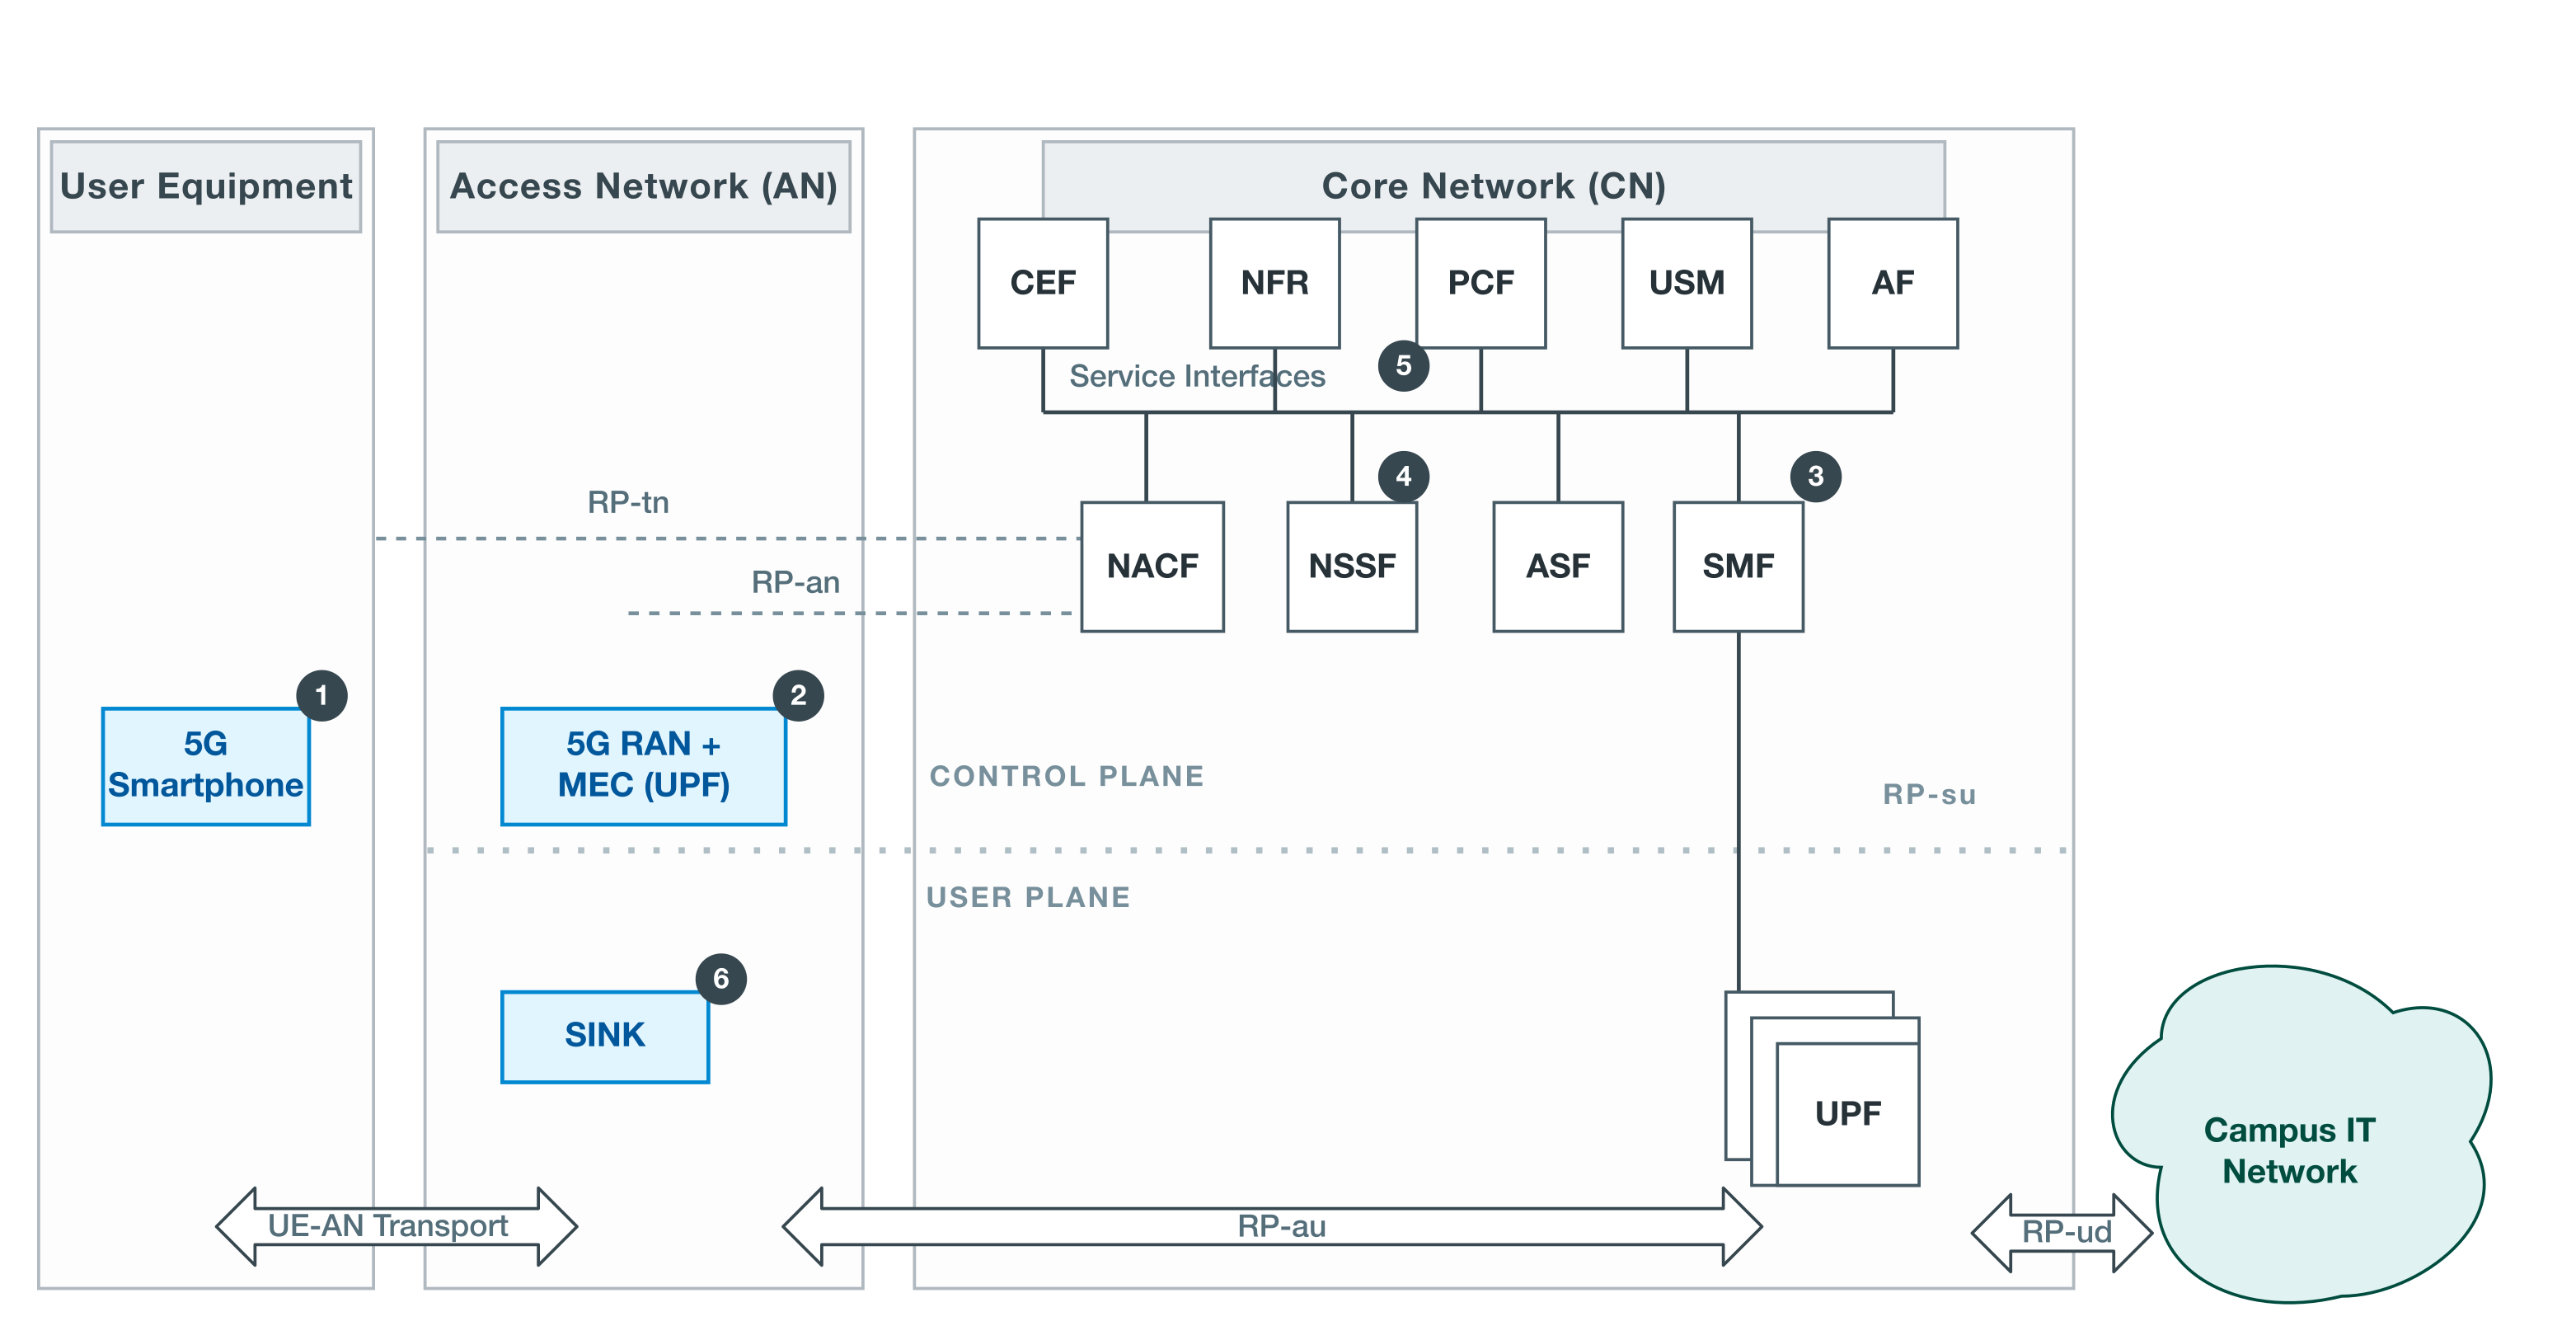
\includegraphics[width=\linewidth]{singh7.png}
    \caption{System architecture of the localized 5G network, illustrating the integration of User Equipment (UE) with the on-premise MEC Server (UPF).}
    \label{fig:5g_implementation}
\end{figure}


\begin{figure*}[h]
    \centering
    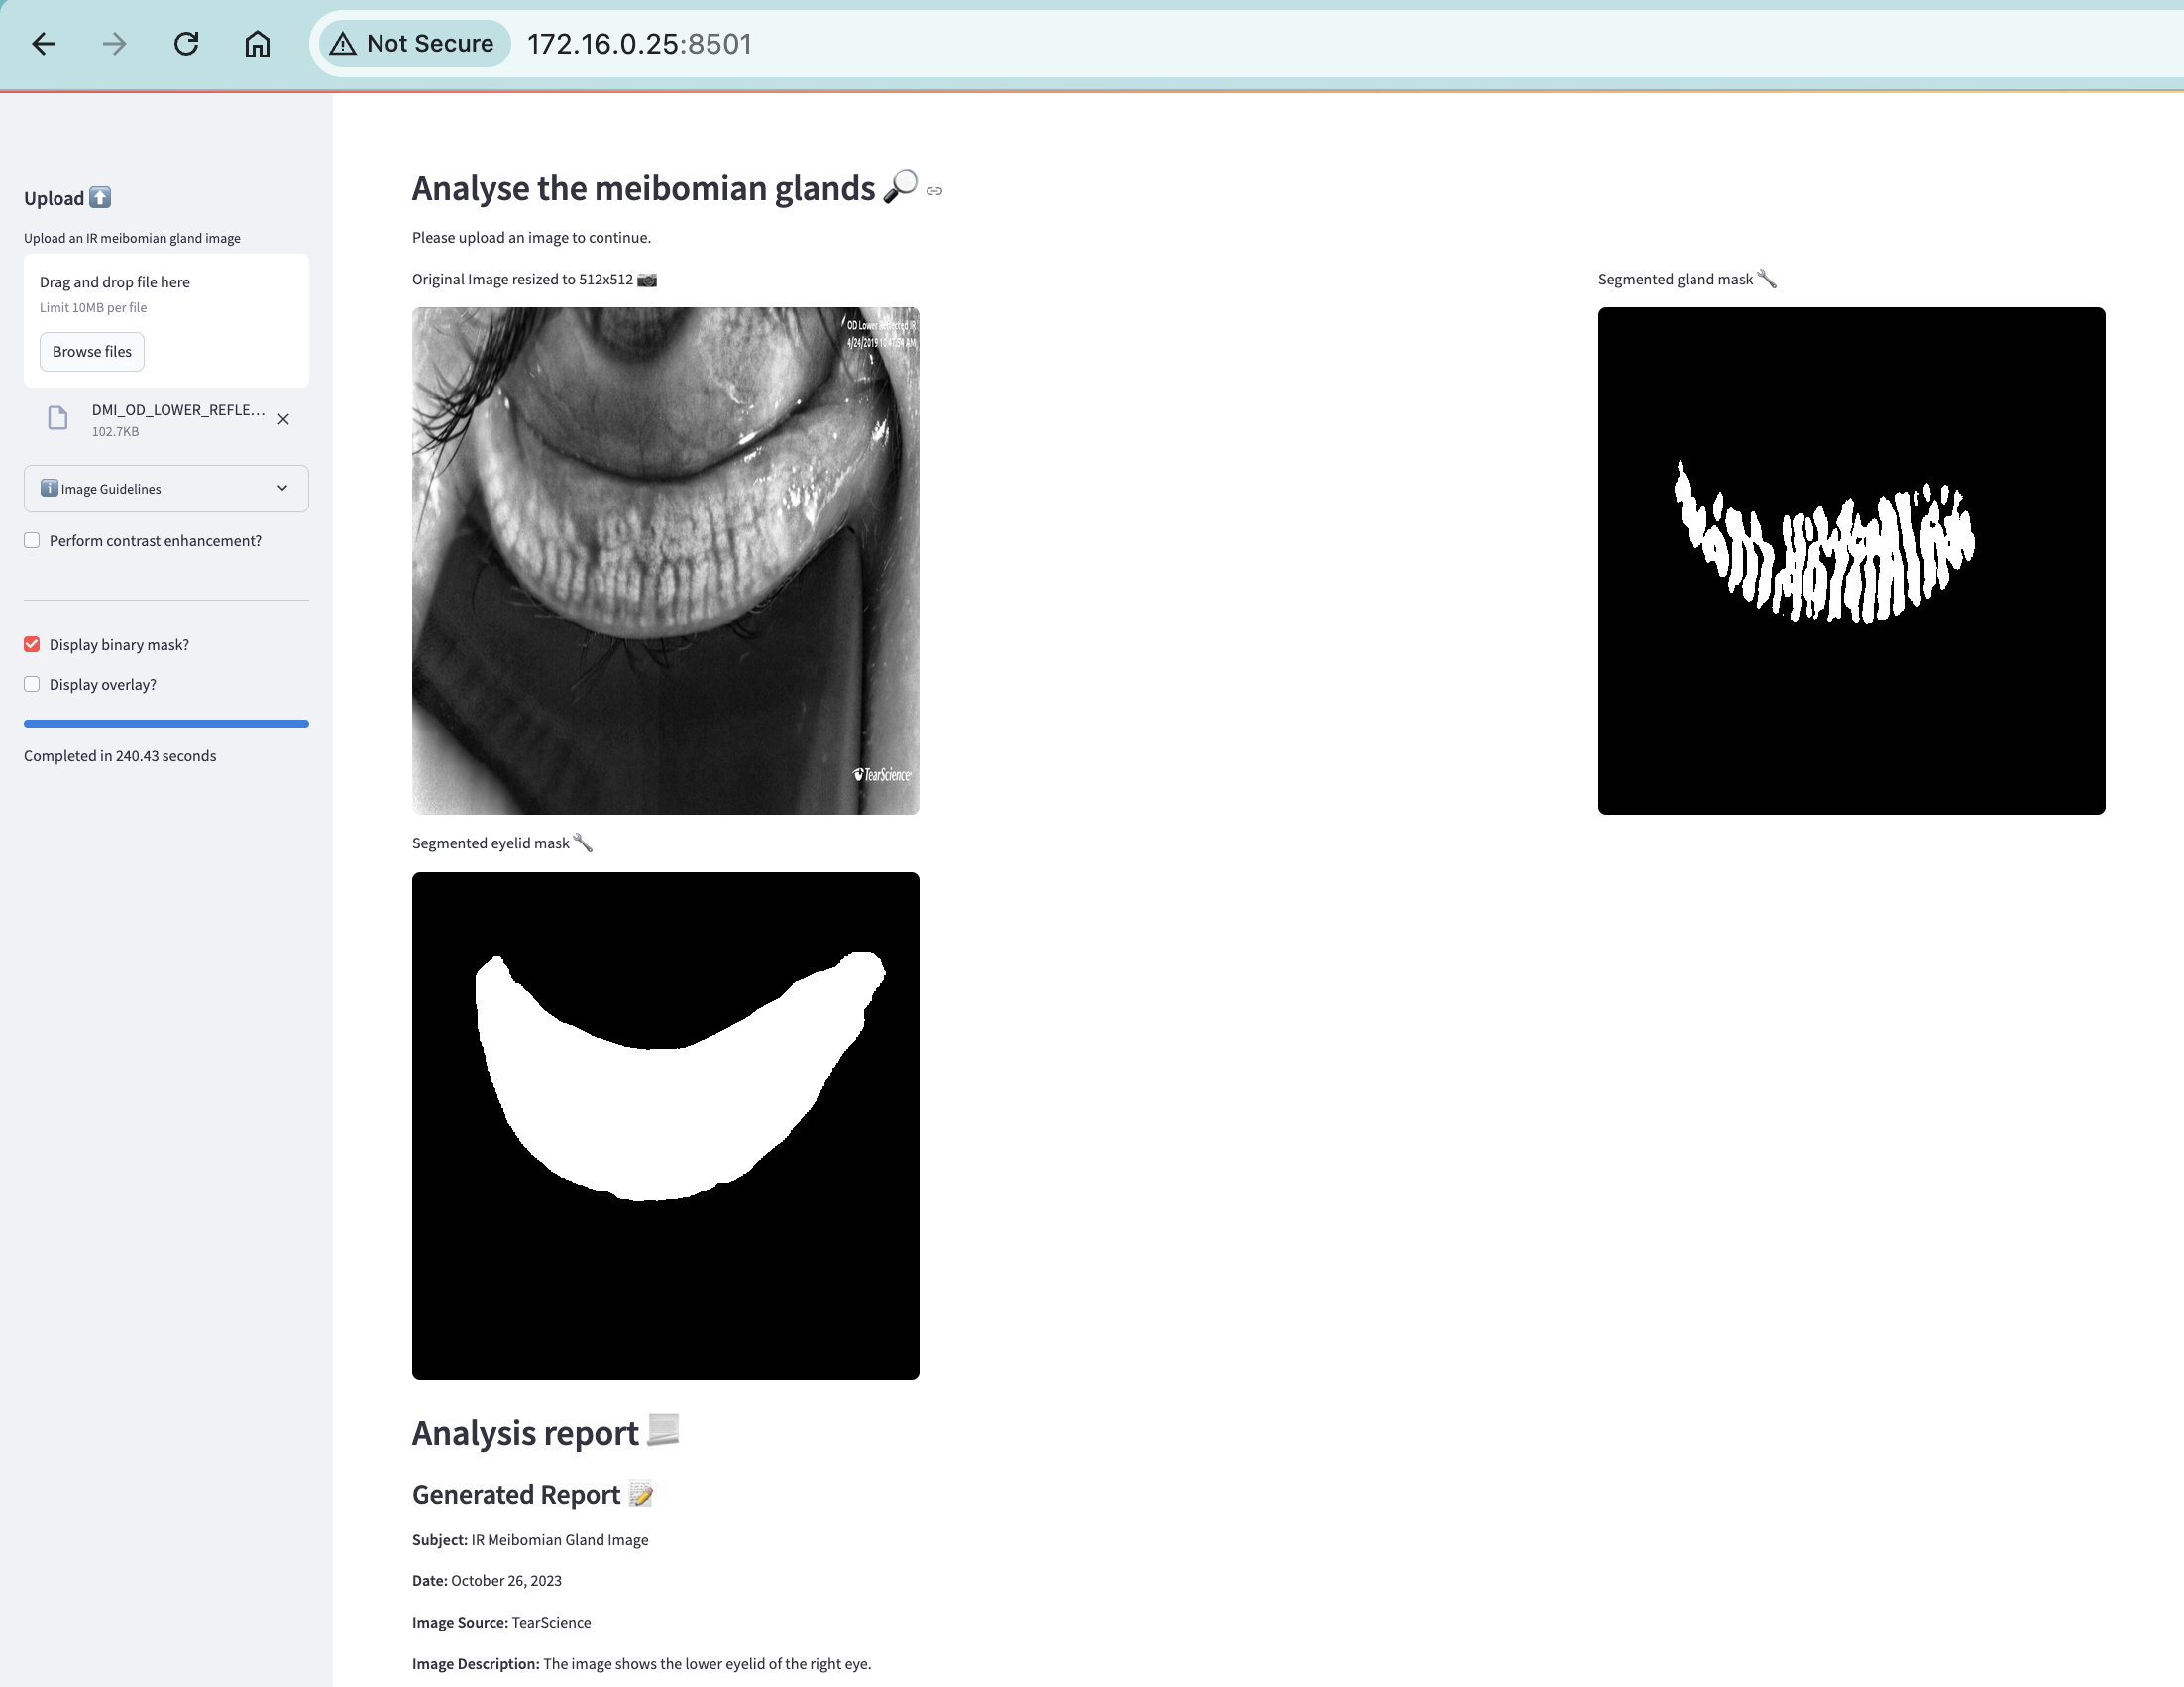
\includegraphics[width=\linewidth]{singh11.png}
    \caption{A screenshot of the user interface of the Digital Twin deployed on an on-premise 5G testbed. The interface allows users to upload meibography images, view the segmentation results and LLM generated summary.}
    \label{fig:user_interface_screenshot}
\end{figure*}

The deep learning pipeline (dual Attention U-Nets and MedGemma) is encapsulated within a Python-based ecosystem on the MEC server.
An interactive frontend is developed as a Streamlit web application serving as the user interface \cite{streamlit}. Streamlit allows rapid rendering of the segmented gland overlays and the MedGemma-generated text grading directly on the web browsers. For the inference pipeline, upon receiving an image query from a UE, the server routes the data sequentially through the eyelid Attention U-Net, the gland Attention U-Net, and finally the MedGemma grading module. Because the Ubuntu server is physically co-located with the UEs, the high bandwidth of the 5G network allows the system to efficiently handle concurrent HTTP requests from multiple UEs e.g. smartphones, maintaining real-time feedback loops essential for an interactive Digital Twin environment. Fig. \ref{fig:5g_implementation} shows the components of the 5G test bed. User equipments (UE) like 5G smartphones are used as source of data. The data is transmitted wirelessly to the access network through 5G radio access network (5G RAN). From the control plane the data is routed to the application hosted in the user plane function (UPF). The edge modules are deployed in the user plane. The result of the system is sent to the sink which is the user interface. A screenshot of the user interface is shown in fig. \ref{fig:user_interface_screenshot} demonstrating the working of the edge modules and as seen by an user of the Digital Twin.

\section{Results}
%\subsection{Evaluation}
The performance of the proposed Attention U-Net architecture was quantitatively evaluated on the test split (20\%) of the MGD-1k dataset, comprising 189 infrared meibography images. The evaluation focused on two key segmentation tasks: the eyelid boundary and the structures of the   meibomian gland. Table 1 shows the performance metrics: Dice Score, Intersection-over-Union (IoU), Precision, Recall and F1-Score for both segmentation modules. The eyelid region of interest segmentation task achieved a Dice Score of 0.961 and IoU of 0.926. This indicates the model’s robustness in accurately delineating the tarsal region. For the gland segmentation task, the model achieved a Dice Score of 0.881 and an IoU of 0.790. This indicates strong performance of segmentation despite the fine-grained and irregular morphology of the glands. In addition to these quantitative evaluations, a qualitative visualization of the segmentation result is presented in Figure 6. It displays a sample of the input infrared image, the predicted binary mask of the eyelid region, and the binary mask of the meibomian glands. This visual result shows that the model effectively isolates anatomical structures of the glands.

\begin{table}[h]
\centering
\caption{Evaluation metrics of Attention U-Net on MGD-1k test set (20\% split)}

\begin{tabular}{lcc}
\hline
\textbf{Metric} & \textbf{Eyelid (mean $\pm$ 95\% CI)} & \textbf{Gland (mean $\pm$ 95\% CI)} \\
\hline
Dice Score  & $95.58 \pm 0.80$ & $74.28 \pm 5.19$ \\
IoU         & $91.71 \pm 1.29$ & $59.69 \pm 5.98$ \\
Precision   & $95.80 \pm 1.23$ & $75.39 \pm 5.04$ \\
Recall      & $95.52 \pm 0.59$ & $75.58 \pm 10.07$ \\
\hline
\label{tab:eval-metrics}
\end{tabular}
\end{table}



\begin{table}[h]
\centering
\caption{Gland Segmentation}
\begin{tabular}{llllll}
   Loss Function & Dice  & IoU & Precision & Recall \\
   \hline
   BCE & 0.7548& 0.6089& 0.8329& 0.6990\\
   Dice & 0.7759& 0.6368& 0.7336& 0.8355\\
   TVERSKY & 0.7497& 0.6037& 0.6427& 0.9149\\
   FOCAL & 0.7643& 0.6210& 0.8027& 0.7401\\
   COMBO&0.7562&0.6116&0.8015&0.7270\\
   CONTOUR&0.5913&0.4228&0.7122&0.5113\\
   DICEBCE&0.7748&0.6351&0.7533&0.8090\\
   IOUBCE&0.7750&0.6356&0.7522&0.8098\\
\label{tab:gland-eval-metrics}
\end{tabular}
\end{table}


\begin{table}[h]
\centering
\caption{Eyelid Segmentation}
\begin{tabular}{llllll}
   Loss Function & Dice  & IoU & Precision & Recall \\
   \hline
   BCE & 0.9613& 0.9261& 0.9651& 0.9586\\
   Dice & 0.9580& 0.9201& 0.9725& 0.9447\\
   TVERSKY & 0.9579& 0.9198& 0.9462& 0.9711\\
   FOCAL & 0.9614& 0.9262& 0.9589& 0.9651\\
   COMBO&0.9625&0.9282&0.9694&0.9566\\
   CONTOUR&0.9513&0.9428&0.9712&0.9531\\
   DICEBCE&0.9545&0.9138&0.9467&0.9640\\
   IOUBCE&0.9545&0.9138&0.9467&0.9640\\
\label{tab:eyelid-eval-metrics}
\end{tabular}
\end{table}

\begin{figure}[h]
    \centering
    \begin{subfigure}{0.32\columnwidth}
        \centering
        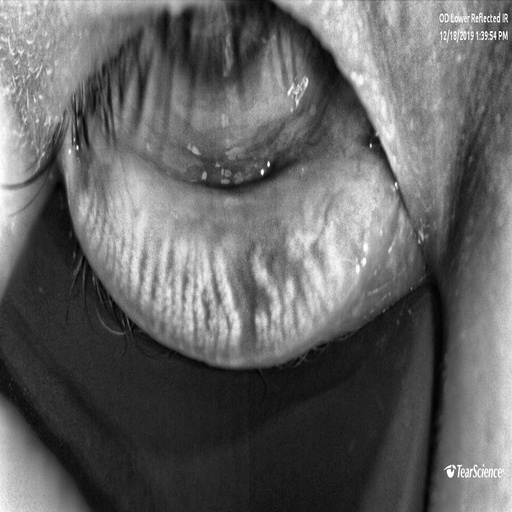
\includegraphics[width=\linewidth]{singh8.jpg}
        \caption{IR image}
        \label{fig:meibography_image_test_sample}
    \end{subfigure}
    \begin{subfigure}{0.32\linewidth}
        \centering
        
\includegraphics[width=\linewidth]{singh9.jpg}
        \caption{Eyelid mask}
        \label{fig:eyelid_mask_test_sample}
    \end{subfigure}
    \begin{subfigure}{0.32\linewidth}
        \centering
        
\includegraphics[width=\linewidth]{singh10.jpg}
        \caption{Gland mask}
        \label{fig:gland_mask_test_sample}
    \end{subfigure}

    \caption{Input image and results of segmentation. (a) Infrared meibography image. (b) Eyelid mask region of interest. (c) Gland mask indicating the precise glandular structure.}
    \label{fig:segmentation_results}
\end{figure}


\begin{figure*}[h]
    \centering
    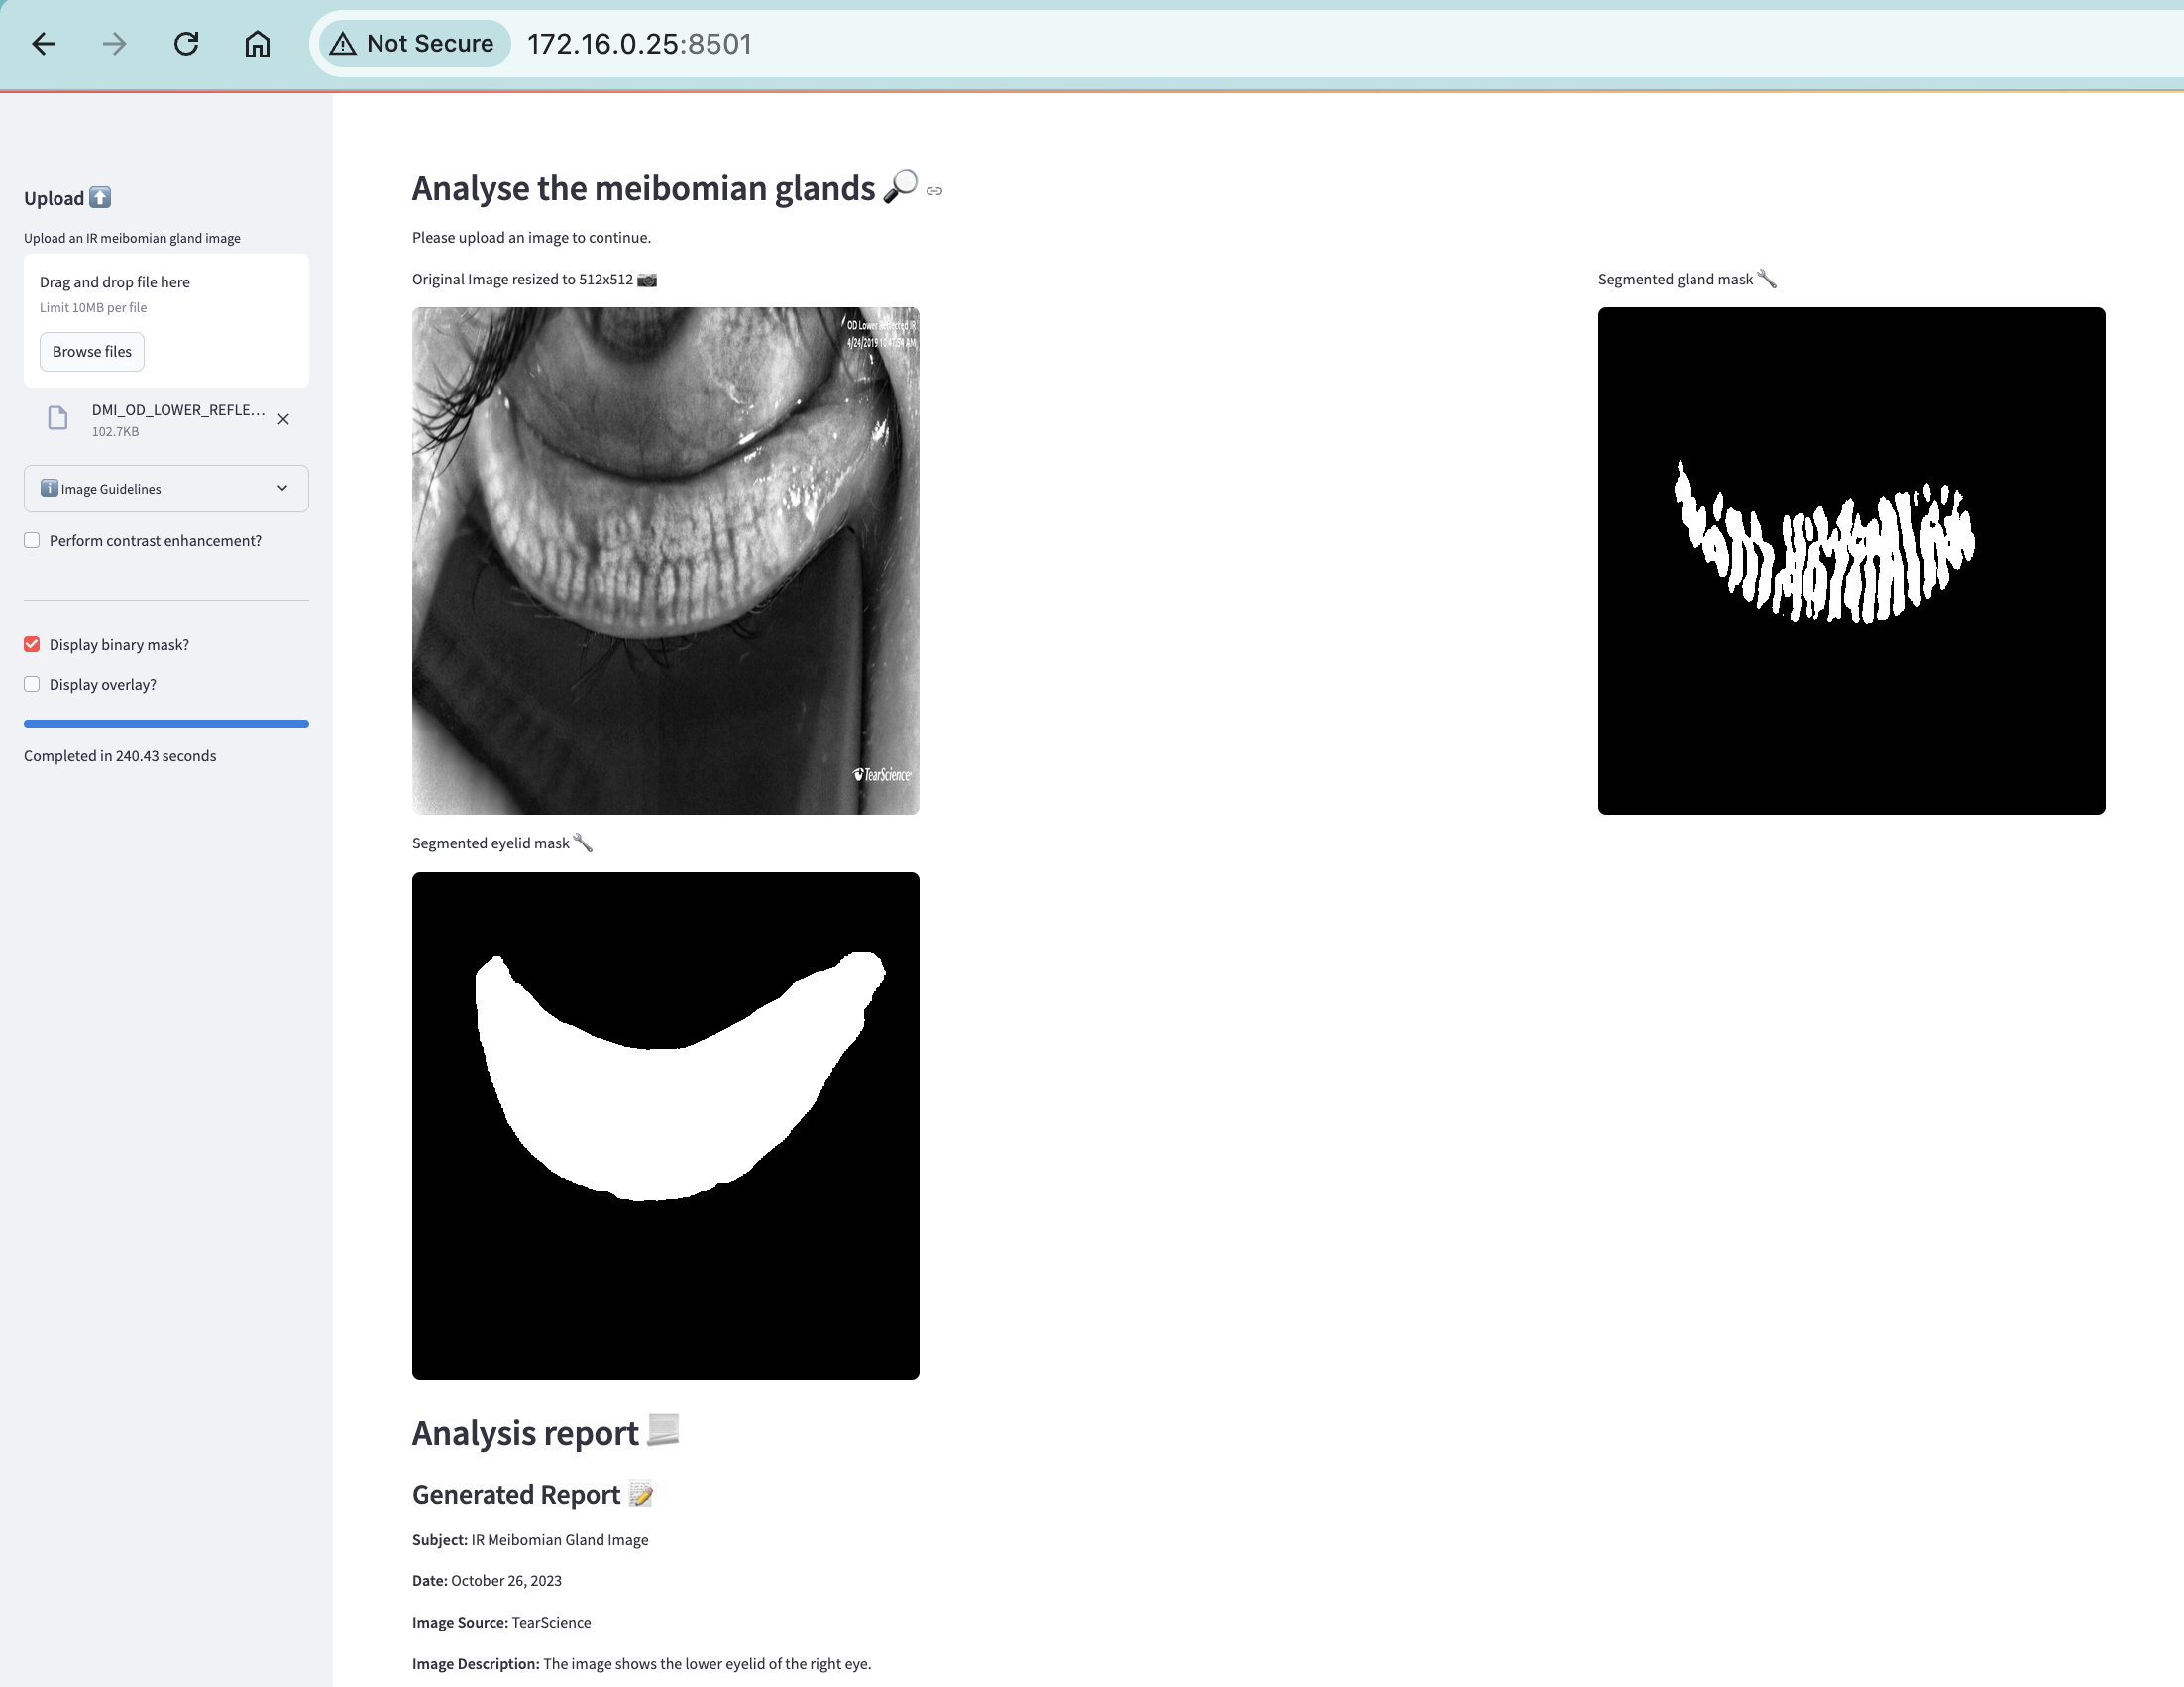
\includegraphics[width=\linewidth]{singh11.png}
    \caption{A screenshot of the user interface of the Digital Twin deployed on an on-premise 5G testbed. The interface allows users to upload meibography images, view the segmentation results and LLM generated summary.}
    \label{fig:user_interface_screenshot}
\end{figure*}


\clearpage
\section{Conclusions}

%\textcolor{red}{Visualization plays a key role in extracting meaningful insights from the dataset. Some visualization recommendation approaches rely on existing knowledge to obtain the recommendations, but they are often required to be processed from scratch to recommend the visualization for incremental data. Therefore, we proposed the IVR\_I approach, which is unique and recommends the visualization for the incremental added over time based on the user's specific requirements provided as Intent. There are existing NLDR approaches for visualizing the high-dimensional data, but they fail to capture the cluster information. To address this, we proposed $HM\_QCv$ that preserves the local structure, global structure, and cluster information. }

The subjectivity in the analysis of meibomian gland dysfunction using infrared meibography due the variability in gland morphology and clinical assessment can be reduced by developing a baseline model. We have used U-Net to segment the glands and an LLM to summarize and grade the glands. The integration of computer vision based image segmentation with an LLM helps in producing easy to understand reports and interactive processing of the images. The developed segmentation models and LLM reporting modules are deployed in the 5G MEC testbed.

\section{Future Work}

%We plan to propose an Agentic AI based Digital Twin to provide a solution to the Meibomian Gland Analysis using infrared meibography. The agentic orchestrator will call the segmentation and reporting modules as tools and perform the meibography analysis.

The future work aims to propose and develop an Agentic AI-based Digital Twin framework for automated meibomian gland analysis using infrared meibography. The proposed framework will incorporate an agentic orchestrator capable of coordinating the execution of the previously developed semantic segmentation and LLM-based reporting modules as callable tools. Based on the input meibography images and the outputs generated by these modules, the orchestrator will manage the analysis workflow and facilitate the generation of structured meibography assessment reports. The framework will be investigated as an integrated approach to intelligent meibomian gland analysis, with emphasis on modularity, automated workflow orchestration, and the integration of AI-based analysis capabilities within a Digital Twin environment.

\bibliography{references}
\bibliographystyle{ieeetr}

\end{document}